\documentclass[11pt, a4paper]{article}
\usepackage[utf8]{inputenc}
\usepackage{amsmath, amssymb}
\usepackage{graphicx}
\usepackage{booktabs}
\usepackage{geometry}
\geometry{margin=1in}

\title{\textbf{Empirical Observation of Transient Arbitrage Phase Transitions}}
\author{Songgun Lee \\ \textit{Department of Physics, UC Santa Barbara}}
\date{\today}

\begin{document}
\maketitle

\section{Empirical Results from Edge Node}
The following data represents the continuous aggregation of our edge-computing node, capturing the maximum dislocation events across a heavily monitored timeframe.

\begin{table}[h]
\centering
\caption{Summary Statistics of Maximum Observed Dislocation by Asset}
\vspace{0.2cm}
\begin{tabular}{l | r | r}
\textit{Asset Pair} & \textit{Max Gross Profit (\%)} & \textit{Mean Kimchi Premium (\%)} \\
\hline
XRP & 0.2545 & 0.2906 \\
ADA & 0.1522 & 0.3213 \\
ETH & 0.1380 & 0.2915 \\
SOL & 0.0287 & 0.2907 \\
DOGE & -0.1189 & 0.3255 \\
\end{tabular}
\end{table}

\begin{figure}[h]
    \centering
    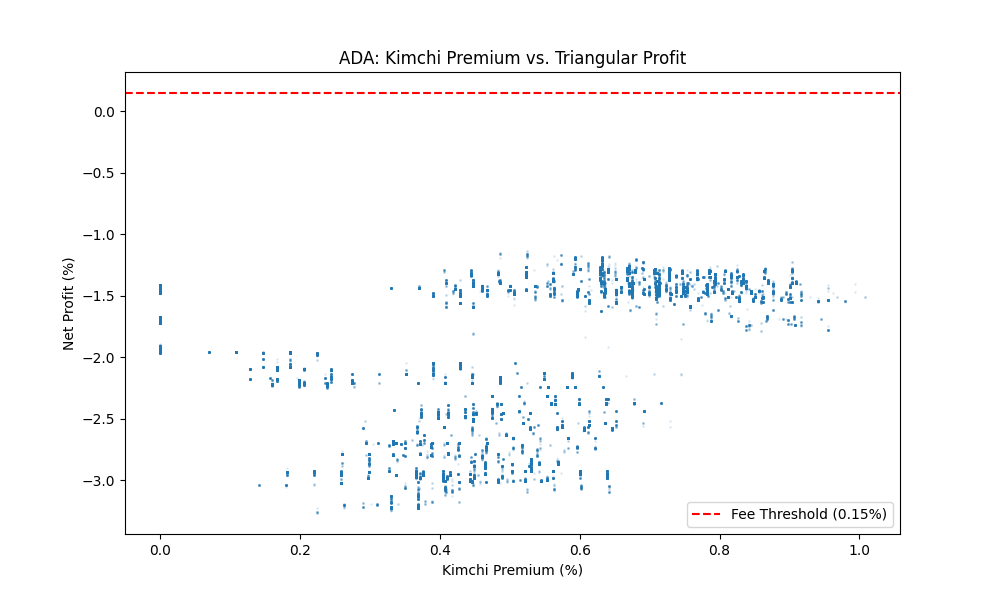
\includegraphics[width=0.85\textwidth]{ada_compressed_analysis.png}
    \caption{Correlation between the Kimchi Premium and Triangular Net Profit (1-Minute Intervals).}
\end{figure}

\end{document}
